\documentclass{article}

\title{Square joy: pre-order}
\subtitle{Restoring a binary tree from its pre-order traversal.}
\reddit{https://www.reddit.com/r/apljk/comments/v5cr09/blog_post_square_joy_preorder/}
\date{2022-06-05}
\modified{2022-06-05}

\keyword{j}
\keyword{arrays}
\keyword{puzzles}

\begin{document}
\section*
In this article, we will solve another programming puzzle using an array programming language, \href{https://www.jsoftware.com/}{J}.
We will play with a data structure that is rarely associated with arrays: a binary tree.
Our goal is to solve the problem using only flat arrays and high-level array transformations.

\section{the-problem}{The problem: recover a binary tree}

Given two sequences of distinct values, \code{inorder} and \code{preorder},
where \code{inorder} is an \href{https://en.wikipedia.org/wiki/Tree_traversal#In-order,_LNR}{in-order traversal} of a binary tree,
and \code{preorder} is a \href{https://en.wikipedia.org/wiki/Tree_traversal#Pre-order,_NLR}{pre-order traversal} of the \em{same} tree, recover the tree structure.

For example, if our inputs are the following sequences

\begin{tabular*}{r l}
\code{inorder} & \code{A P L J K Q F U N} \\
\code{preorder} & \code{Q P A J L K U F N} \\
\end{tabular*}

then the corresponding tree has the shape depicted on the figure below.

\begin{figure}[grayscale-diagram]
\marginnote{mn-tree-example}{
  A tree corresponding to inputs \code{inorder = A P L J K Q F U N} and \code{preorder = Q P A J L K U F N}.
  We will use this tree as our primary example throughout the article.
}
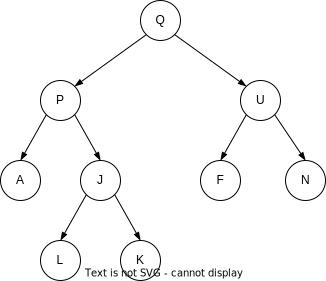
\includegraphics{/images/07-problem-tree.svg}
\end{figure}

\section{vectorizing-the-problem}{Vectorizing the problem}
\epigraph{
  A problem well stated is a problem half solved.
}{John Dewey}

The way we represent the inputs and outputs of our problem shapes our approach to a solution.

Our inputs, \code{inorder} and \code{preorder}, are already arrays.
However, there is something peculiar about these arrays: they contain the same values, or, in math terms, \code{preorder} is a \em{permutation} of \code{inorder}.
We can eliminate this redundancy by compressing the inputs to a single numeric array: the permutation that turns \code{inorder} into \code{preorder}.
A primitive J operation, dyadic \href{https://code.jsoftware.com/wiki/Vocabulary/idot#dyadic}{\code{i.} (index of)}, transforms the original inputs to the more convenient and compact permutation form.

\begin{verbatim}[j]
    'APLJKQFUN' i. 'QPAJLKUFN'
5 1 0 3 2 4 7 6 8
\end{verbatim}

\begin{figure}[grayscale-diagram]
\marginnote{mn-tree-perm}{
  The example tree after we changed node labels to be integers corresponding to the in-order traversal.
}
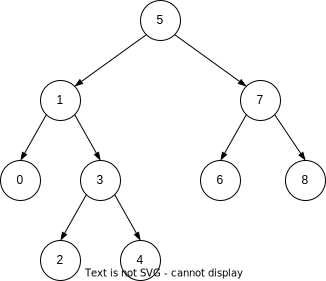
\includegraphics{/images/07-problem-tree-digits.svg}
\end{figure}

The next step is to decide on the tree representation.
There are two popular representations in the array community: depth vector and parent vector.

\subsection{depth-vector}{Depth vector}

The depth vector is a tree representation that you often see in graphical user interfaces, such as text editors displaying the project file structure.
This representation consists of the vector of nodes as they appear in the pre-order traversal and the vector of corresponding node depths.
\begin{verbatim}[j]
    T =. 5 1 0 3 2 4 7 6 8
    D =. 0 1 2 2 3 3 1 2 2
\end{verbatim}

The pre-order vector specifies the vertical order of the nodes; the depth vector specifies how far these nodes lie horizontally.
\begin{verbatim}[j]
   ((D>:/H) + (T+1) * D=/ H =. i.1+>./D) { ' .APLJKQFUN'
Q
.P
..A
..J
...L
...K
.U
..F
..N
\end{verbatim}

This representation has many benefits, but it is not convenient for our problem.

\subsection{parent-vector}{Parent vector}

The \href{https://dl.acm.org/doi/10.1145/586058.586060}{parent vector} is an array mapping nodes to their parents.
Technically, the root node does not have a parent, but many algorithms become more elegant if we extend the definition of parent to work for the root node as well: we declare that the parent of the root node is the root node itself.

Array \code{1 5 3 1 3 5 7 5 7} is the parent vector encoding for our example tree.
\begin{verbatim}[j]
    P =. 1 5 3 1 3 5 7 5 7
\end{verbatim}

Let us play with this representation a bit to understand it better.
We will use a couple of J primitives: \href{https://code.jsoftware.com/wiki/Vocabulary/icapdot}{\code{I.} (indices)} returning the indices of set bits in a boolean mask, and \href{https://code.jsoftware.com/wiki/Vocabulary/edot#dyadic}{\code{e.} (member in)} returning a boolean mask that has the shape of the left argument and has bits set for items that appear in the right argument.

Let us find the\sidenote{mn-forest}{Parent vector representation also works for \href{https://en.wikipedia.org/wiki/Tree_(graph_theory)#Forest}{forests}.} tree root, the node that is its parent.
\begin{verbatim}[j]
    P = i.#P
0 0 0 0 0 1 0 0 0

    I. (P = i.#P)
5
\end{verbatim}

How about finding direct children of node \code{3}?
Those are nodes having \code{3} as their parent.
\begin{verbatim}[j]
    I. P = 3
2 4
\end{verbatim}

How about finding all leaves?
Those are nodes that do not appear in the parent vector.
\begin{verbatim}[j]
    -. (i.#P) e. P
1 0 1 0 1 0 1 0 1

   I. -. (i.#P) e. P
0 2 4 6 8
\end{verbatim}

The parent vector representation does not distinguish right children from left children.
However, we label our nodes in-order, so there is a simple way to tell the direction: nodes with indices lower than their parents are left children, and nodes with higher indices are right children.
\begin{verbatim}[j]
   NB. all left children
   I. (i.#P) < P
0 1 2 6

   NB. all right children
   I. (i.#P) > P
3 4 7 8
\end{verbatim}

Parent vector gives us a simple, elegant, and self-contained tree representation.
It is perfect for solving the problem.

We have decided on the form of our solution: a monadic function that accepts a permutation and returns a parent vector of the same shape.

\section{a-solution}{A solution}
\subsection{left-children}{Finding left children}

Where should we start?
I like to start by finding a way to visualize the data.
One way to visualize a permutation is to draw a table showing how it scrambles items in space.

\begin{verbatim}[j]
    T =/ i.#T
0 0 0 0 0 1 0 0 0
0 1 0 0 0 0 0 0 0
1 0 0 0 0 0 0 0 0
0 0 0 1 0 0 0 0 0
0 0 1 0 0 0 0 0 0
0 0 0 0 1 0 0 0 0
0 0 0 0 0 0 0 1 0
0 0 0 0 0 0 1 0 0
0 0 0 0 0 0 0 0 1
\end{verbatim}

Look at the ones!
If you squint a bit, you will see that they form a picture of the tree we started with\sidenote{sn-ones-tree}{The reason is obvious in hindsight, but I was quite surprised when I drew the picture for the first time.}.
Let us use the \href{https://code.jsoftware.com/wiki/Vocabulary/gtco#dyadic}{\code{>:} (greater or equal)} verb instead of equality in the table and multiply each column by T.

\begin{code}[j]
    T * T >:/ i.#T
5 5 5 5 5 \u{5} 0 0 0
1 \u{1} 0 0 0 0 0 0 0
\u{0} 0 0 0 0 0 0 0 0
3 3 3 \u{3} 0 0 0 0 0
2 2 \u{2} 0 0 0 0 0 0
4 4 4 4 \u{4} 0 0 0 0
7 7 7 7 7 7 7 \u{7} 0
6 6 6 6 6 6 \u{6} 0 0
8 8 8 8 8 8 8 8 \u{8}
\end{code}

This table has an interesting property: if we look at the places where ones used to be (underscored), the value right above that place is either zero (for all right children) or the parent in the tree (for all left children).
Why is that?

Let us inspect the structure of a pre-order permutation vector.
After adding a node index to the vector, we descend into the left child (if there is one).
That left child will always follow the parent in the pre-order vector.
Left children have indices lower than the index of their parent because we assign indices according to in-order traversal.
A simple pattern emerges: if we see numbers \math{a} and \math{b} next to each other, and \math{a > b}, then \math{a} is the parent of \math{b}.

\begin{figure}[grayscale-diagram]
  \marginnote{mn-left-children}{The left children follow a pattern in a pre-order vector: whenever a smaller node index follows a larger one, the larger index must be the parent of the smaller.}
  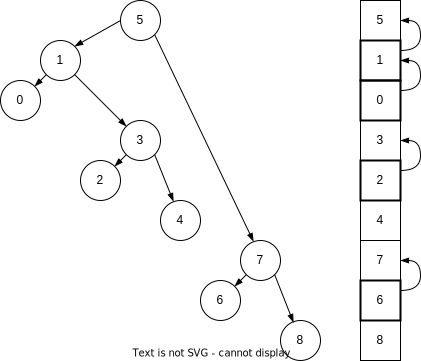
\includegraphics{/images/07-left-children.svg}
\end{figure}

Let us put this observation into code.
We shift the input vector to the right, filling the space on the left with the first value in the vector (the root node).
We then compute \math{Shifted × (T ≤ Shifted)}.

\begin{verbatim}[j]
    NB. get the head of the vector
    {.T
5
\end{verbatim}

\begin{verbatim}[j]
    NB. shift to the right, filling the space with the head
   _1 |.!.({.T) T
5 5 1 0 3 2 4 7 6
\end{verbatim}

\begin{verbatim}[j]
    NB. compute T <= Shifted
    T <: _1 |.!.({.T) T
1 1 1 0 1 0 0 1 0
\end{verbatim}
\begin{verbatim}[j]
    NB. L = Shifted * (T <= Shifted)
    ] L =. T (<: * ]) _1 |.!.({.T) T
5 5 1 0 3 0 0 7 0
\end{verbatim}
\begin{verbatim}[j]
    NB. the parent of node 5 is 5, the parent of node 1 is 5, etc.
    T,:L
5 1 0 3 2 4 7 6 8
5 5 1 0 3 0 0 7 0
\end{verbatim}

Array \code{L} is not the correct answer yet: the parents we computed for the right children are zero.

\subsection{right-children}{Finding right children}

To find the parents of the right children, we have to look closely at the pre-order vector again.
When we construct the vector, we first append the parent, follow the whole left subtree, and then goes the right child.
All nodes in the left subtree have indices smaller than the parent, and the right child has an index larger than the parent.

\begin{figure}[grayscale-diagram]
  \marginnote{mn-left-children}{The right children follow a pattern in a pre-order vector: their parent node is the largest index earlier in the vector smaller than their index.}
  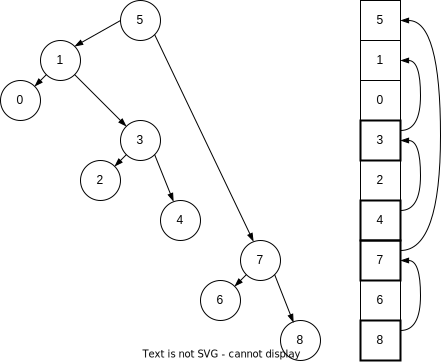
\includegraphics{/images/07-right-children.svg}
\end{figure}

This observation gives us an algorithm: we need to find the largest value to the left smaller than the node for each position in the array.
The simplest way to express this algorithm in J is to use the \href{https://code.jsoftware.com/wiki/Vocabulary/bslash}{\code{\}}} adverb (prefix scan).
We look at each prefix and find the largest value in that prefix that is smaller than the last element of the prefix.
Let us take the prefix \code{5 1 0 3} as an example.

\begin{verbatim}[j]
    NB. {: computes the last element of an array
    {: 5 1 0 3
3

    NB. compute the boolean mask of items smaller than the last element
    (] < {:) 5 1 0 3
0 1 1 0

    NB. filter out elements according to the boolean mask
    ((] < {:) # ]) 5 1 0 3
1 0

    NB. find the maximum
    (>./ @ ((] < {:) # ])) 5 1 0 3
1
\end{verbatim}

Let us now apply our composite verb to each successive prefix of the pre-order array.

\begin{verbatim}[j]
    NB. __ means "negative infinity".
    ] R =. (>./ @ ((] < {:) # ]))\ T
__ __ __ 1 1 3 5 5 7
\end{verbatim}

\begin{verbatim}[j]
    NB. node 5 has no parent, the parent of node 3 is 1, etc.
    T,:R
 5  1  0 3 2 4 7 6 8
__ __ __ 1 1 3 5 5 7
\end{verbatim}

Array \code{R} has incorrect values for parents of all left children.
We shall deal with this issue in the next section.

\subsection{computing-parent-vector}{Computing the parent vector}

We have two ways to compute the parents: one works for left children (let us call it the \em{L-algorithm}), and another works for right children (the \em{R-algorithm}).
How do we combine these results?

Note that array \code{L} had zeros for all right children. 
Also, note that the L-algorithm produces larger values than the R-algorithm: the L-algorithm looks for \em{larger} nodes to the left of each position, while the R-algorithm looks for \em{smaller} nodes.
So taking the maximum of arrays \math{L} and \math{R} gives us the correct answer.

\begin{verbatim}[j]
    L >. R
5 5 1 1 3 3 5 7 7

    NB. node 5 has parent 5, node 1 has parent 5, etc.
    T ,: L >. R
5 1 0 3 2 4 7 6 8
5 5 1 1 3 3 5 7 7
\end{verbatim}

We are not there yet: the parent vector appears scrambled because it mirrors the pre-order permutation.
We need to enumerate parents according to the in-order traversal by applying the inverse permutation to get the final answer.

\begin{verbatim}[j]
    NB. Compute the inverse permutation for T
    T i. i.#T
2 1 4 3 5 0 7 6 8
\end{verbatim}

To apply a permutation, we use it as an index of the array we want to permute\sidenote{sn-permute}{Applying permutations is a common operation in array programming, so J has a primitive function for that, \href{https://code.jsoftware.com/wiki/Vocabulary/ccapdot#dyadic}{\code{C.} (permute)}.}.
\begin{verbatim}[j]
    NB. apply the inverse permutation to the scrambled parents
    (T i. i.#T) { L >. R
1 5 3 1 3 5 7 5 7
\end{verbatim}

We got our answer.
Let us extract our little exploration into a function.
\begin{verbatim}[j]
recover_tree =. {{
  L =. y (<: * ]) _1 |.!.({.y) y
  R =. (>./ @ ((] < {:) # ]))\y
  (y i. i.#y) { L >. R
}}
\end{verbatim}

Same function in tacit form:
\begin{verbatim}[j]
recover_tree =. (i. i.@#) { ((<: * ]) ({. , }:))~ >. >./@((] < {:) # ])\
\end{verbatim}

\section{c-solution}{Bonus: stinking loop solution}

While playing with J, we learned that we need only one permutation as input, and that we can represent the result as a flat array of parents.
Let us apply this knowledge to get an efficient and short solution in C.

We will use recursion to solve the problem.
Let us consider a traversal of a subtree spanning from node \math{L} to node \math{R} (\math{R} excluded).
The first item in the pre-order array gives the root \math{P} of that subtree.
\math{P - L} nodes to the left of \math{P} (indices \math{L..P}) form the left subtree, and \math{R - P} nodes to the right of \math{P} (indices \math{P+1..R}) constitute the right subtree.
We handle those subtrees recursively, assigning \math{P} as their root.

Let us look at the example, \code{5 1 0 3 2 4 7 6 8}.
The first node in the array is the root, \code{5}.
It divides the rest of the vector into two sections forming the left and the right subtrees correspondingly: nodes \code{0 1 2 3 4} (five nodes in total) and nodes \code{6 7 8} (three nodes in total).
We can compute these subtrees recursively and assign \code{5} as the root of these subtrees.

\begin{figure}[grayscale-diagram]
  \marginnote{mn-loop-solution}{The run of the recursive parent search algorithm for the first two layers of the example tree.}
  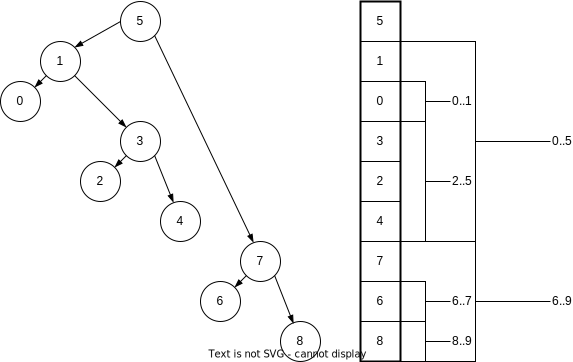
\includegraphics{/images/07-loop-solution.svg}
\end{figure}
\begin{figure}
  \marginnote{mn-loop-solution-code}{
    A C implementation of the recursive algorithm for computing the parent vector.
    \code{Pre} is the pre-order traversal array, \code{P} is the output array of parents, \code{N} is the number of tree nodes.
  }
\begin{code}[c]
static void restore_range(int Pre[], int P[], int L, int R, int V) {
    if (L >= R) return;
    P[Pre[0]] = V;
    restore_range(Pre + 1, P, L, Pre[0], Pre[0]);
    restore_range(Pre + Pre[0] - L + 1, P, Pre[0] + 1, R, Pre[0]);
}

void restore_tree(int Pre[], int P[], int N) {
    if (N > 0) restore_range(Pre, P, 0, N, Pre[0]);
}
\end{code}
\end{figure}

Note that this code is inherently polymorphic: it does not care about the type of elements we store in the tree.

\section{where-to-go-next}{Where to go next}
\begin{itemize}
  \item Discuss this article on \href{https://www.reddit.com/r/apljk/comments/v5cr09/blog_post_square_joy_preorder/}{Reddit}.
  \item Solve this problem on \href{https://leetcode.com/problems/construct-binary-tree-from-preorder-and-inorder-traversal/}{Leetcode}.
  \item
    Solve a similar problem: recover a tree from its in-order and post-order traversals.
    Hint: all of the tricks discussed in this article will work after changing the direction.
  \item Read the previous "square joy" article, \href{/posts/04-square-joy-trapped-rain-water.html}{trapped rainwater}.
  \item Watch Aaron Hsu's talk, \href{https://www.youtube.com/watch?v=hzPd3umu78g}{High-performance Tree Wrangling, the APL way}.
  \item Read Aaron Hsu's dissertation, \href{https://scholarworks.iu.edu/dspace/handle/2022/24749}{A data parallel compiler hosted on GPU}.
    It goes deep into tree representations and conversions between these representations.
    There are many exciting algorithms on the parent vector representation, too.
  \item Listen to the \href{https://arraycast.com/}{Arraycast} podcast.
\end{itemize}
\end{document}
